\chapter{Numerical Methods}
\begin{stbox}{General Information}
    \begin{itemize}
        \item The parity of the degree of a real polynomial is the same as that of its number of real roots.
        \item Let the real polynomial \(p\) given by \(p(x)=a_{2n}x^{2n}+a_{2n-1}x^{2n-1}+\dots+a_0\) have coefficients \(a_n>0\) and \(a_0<0\). Then, it has at least one positive and one negative root.
        \item To show that there a continuous function \(f\) attains a root in an interval \([a,b]\), we find two values \(x<y\) in the interval (e.g. \(a<b\)) such that \(f(a)f(b)<0\). i.e. show that \(f\) changes sign in \([a,b]\). Then, \emph{by continuity}, a root of \(f\) must lie in \([a,b]\).
        \item To further show that the root is \emph{unique} in \([a,b]\), it suffices to prove that \(f\) is \emph{strictly} monotone on \([a,b]\).
        \item Suppose we have some function \(f \colon \mathbb{R}\to \mathbb{R}\) with a root \(\alpha\), whose value we want to approximate. There are three ways to obtain this approximation.
        \begin{enumerate}
            \item Linear interpolation on an interval \([a,b]\) containing \(\alpha\). Our approximation is
            \[\frac{a \lvert f(b) \rvert+b \lvert f(a) \rvert}{\lvert f(a) \rvert+\lvert f(b) \rvert}.\]
            \begin{itemize}
                \item The sequence \(\{x_n\}\) of approximations \emph{always} converges to \(\alpha\).
                \item The smaller \(\lvert f''(x) \rvert\) is (i.e. the slower the gradient \(f'(x)\) changes) near \(\alpha\), the faster the rate of convergence.
                \item Error:
                \begin{table}[H]
                    \centering
                    \begin{tabular}{|Sc|Sc|Sc|}
                        \hline
                        Concave/Gradient & Positive & Negative\\
                        \hline
                        Upwards \(\bigcup\) & \textcolor{blue}{underestimation} & \textcolor{red}{overestimation}\\
                        \hline
                        Downwards \(\bigcap\) & \textcolor{red}{overestimation} & \textcolor{blue}{underestimation}\\
                        \hline
                    \end{tabular}
                    \caption{Approximation errors when using linear interpolation.}
                    \label{table:linear-interpolaion}
                \end{table}
                \item See Figure \ref{fig:linear-interpolation} for an illustration.
                \footnotetext{Screw trying to make nice diagonal cells. Pain. Suffering.}
            \end{itemize}
        \end{enumerate}
    \end{itemize}
\end{stbox}
\begin{note}
    At every iteration of linear interpolation, we must ensure that \(\alpha\in [a,x_n]\). Otherwise \(x_n\) may not approximate \(\alpha\). If \(\alpha\notin [a,x_n]\), simply consider \(\alpha\in [x_n,b]\) (or any other suitable interval) instead.
\end{note}
\begin{note}
    It is important to show which interval we are interpolating on, not just the iteratively obtained values. We can present our working using the table below.
    \begin{table}[H]
        \centering
        \begin{tabular}{|Sc|Sc|Sc|Sc|Sc|}
            \hline
            \(a\) & \(f(a)\) & \(b\) & \(f(b)\) & \(\dfrac{a \lvert f(b) \rvert+b \lvert f(a) \rvert}{\lvert f(a) \rvert+\lvert f(b) \rvert}\)\\
            \hline
            \(a\) & \(f(a)>0\) & \(b\) & \(f(b)<0\) & \(x_1\)\\
            \hline
            \(x_1\) & \(f(x_1)>0\) & \(b\) & \(f(b)<0\) & \(x_2\)\\
            \hline
            \(x_1\) & \(f(x_1)>0\) & \(x_2\) & \(f(x_2)<0\) & \(x_3\)\\
            \hline
            \(\vdots\) & \(\vdots\) & \(\vdots\) & \(\vdots\) & \(\vdots\)\\
            \hline
        \end{tabular}
        \caption{Required working for linear interpolation.}
        \label{table:linear-interpolation-presentation}
    \end{table}
\end{note}
\begin{stbox}{}
    \begin{itemize}
        \item[]
        \begin{enumerate}
            \item[2.] Fixed-point Iteration. First select a function \(F \colon \mathbb{R}\to \mathbb{R}\), such that \(F(\alpha)=\alpha\), and choose some initial approximation \(x_0\) to \(\alpha\). Then, we recursively define \(x_{n+1} \coloneq F(x_n)\). We want \(x_n\to \alpha\).
            \begin{itemize}
                \item Convergence behavior
                \begin{table}[H]
                    \centering
                    \begin{tabular}{|Sc|Sc|Sc|Sc|}
                        \hline
                        Behvaior of \(\lvert F'(x) \rvert\) & Converges? & Rate of convergence\\
                        \hline
                        \(\lvert F'(x) \rvert<1\) and is small near \(\alpha\) & \textcolor{green!70!black}{\checkmark} & \textcolor{green!70!black}{fast}\\
                        \hline
                        \(\lvert F'(x) \rvert<1\) but is close to 1 near \(\alpha\) & \textcolor{green!70!black}{\checkmark} & \textcolor{blue}{slow}\\
                        \hline
                        \(\lvert F'(x) \rvert\geq 1\) near \(\alpha\) & \textcolor{red}{\(\times\)} & -\\
                        \hline
                    \end{tabular}
                    \caption{Convergence behavior of fixed-point iterations.}
                    \label{table:fixed-point-iteration}
                \end{table}
                \item See Figure \ref{fig:fixed-point-iteration} for an illustration.
            \end{itemize}
        \end{enumerate}
    \end{itemize}
\end{stbox}
\begin{note}
    We must write out \emph{all} iterations, not just the final two. The working below is sufficient.

    \rule{20cm-137.0549pt}{0.05mm}

    \vspace{0.5\baselineskip} Let \(x_0=\rule{0.5cm}{0.05mm}\) and \(x_{n+1}=F(x_n)\), \(x\geq 0\).
    \begin{align*}
        x_1&=\rule{0.5cm}{0.05mm}\\
        x_2&=\rule{0.5cm}{0.05mm}\\
        &\vdotswithin{=}\\
        x_{m-1}&=\rule{0.5cm}{0.05mm}\\
        x_m&=\rule{0.5cm}{0.05mm}
    \end{align*}
    Therefore, \(\alpha=x_m\) (\(k\) d.p.), since \(f(x_m-0.0\cdots05)f(x_m+0.0\cdots05)=\rule{0.5cm}{0.01mm}<0\).
\end{note}
\begin{stbox}{}
    \begin{itemize}
        \item[]
        \begin{enumerate}
            \item[3.] The Newton-Raphson Method. Let \(\alpha\) be a root of the function \(f\colon \mathbb{R}\to \mathbb{R}\). The Newton-Raphson formula is
            \[x_{n+1}\coloneq x_n-\frac{f(x_n)}{f'(x_n)}.\]
            \begin{itemize}
                \item The Newton-Raphson method fails in the following cases.
                \begin{enumerate}
                    \item The gradient at \(x_0\) is too gentle.
                    \item The gradient changes too rapidly.
                    \item The initial approximation \(x_0\) is too far from the root \(\alpha\).
                    \item There is a turning point between the initial approximation \(x_0\) and the root \(\alpha\).
                    \item There is a point of inflection --- where the concavity changes/the sign of \(f''(x)\) changes.
                \end{enumerate}
                \item Error: 
                \begin{table}[H]
                    \centering
                    \begin{tabular}{|Sc|Sc|Sc|}
                        \hline
                        Concave/Gradient & Positive & Negative\\
                        \hline
                        Upwards \(\bigcup\) & \textcolor{red}{overestimation} & \textcolor{blue}{underestimation}\\
                        \hline
                        Downwards \(\bigcap\) & \textcolor{blue}{underestimation} & \textcolor{red}{overestimation}\\
                        \hline
                    \end{tabular}
                    \caption{Approximation errors when using the Newton-Raphson method.}
                    \label{table:newton-raphson}
                \end{table}
                \item See Figure \ref{fig:newton's-method} for an illustration.
            \end{itemize}
        \end{enumerate}
    \end{itemize}
\end{stbox}
\begin{note}
    We must write out \emph{all} iterations, not just the final two. One way to present our working is as follows.

    \rule{20cm-137.0549pt}{0.05mm}

    \vspace{0.5\baselineskip} Let \(x_0=\rule{0.5cm}{0.05mm}\) and \(x_{n+1}=x_n-\frac{f(x_n)}{f'(x_n)}=\rule{0.5cm}{0.05mm}\)\,, \(x\geq 0\).
    \begin{align*}
        x_1&=\rule{0.5cm}{0.05mm}\\
        x_2&=\rule{0.5cm}{0.05mm}\\
        &\vdotswithin{=}\\
        x_{m-1}&=\rule{0.5cm}{0.05mm}\\
        x_m&=\rule{0.5cm}{0.05mm}
    \end{align*}
    Therefore, \(\alpha=x_m\) (\(k\) d.p.), since \(f(x_m-0.0\cdots05)f(x_m+0.0\cdots05)=\rule{0.5cm}{0.01mm}<0\).
\end{note}
\begin{note}
    Explain whether \(x_0=\rule{0.5cm}{0.05mm}\) is a suitable starting value for using the Newton-Raphson method to find an approximation to \(\alpha\).
    
    \rule{20cm-137.0549pt-25pt}{0.05mm}
    \begin{figure}[H]
        \centering
        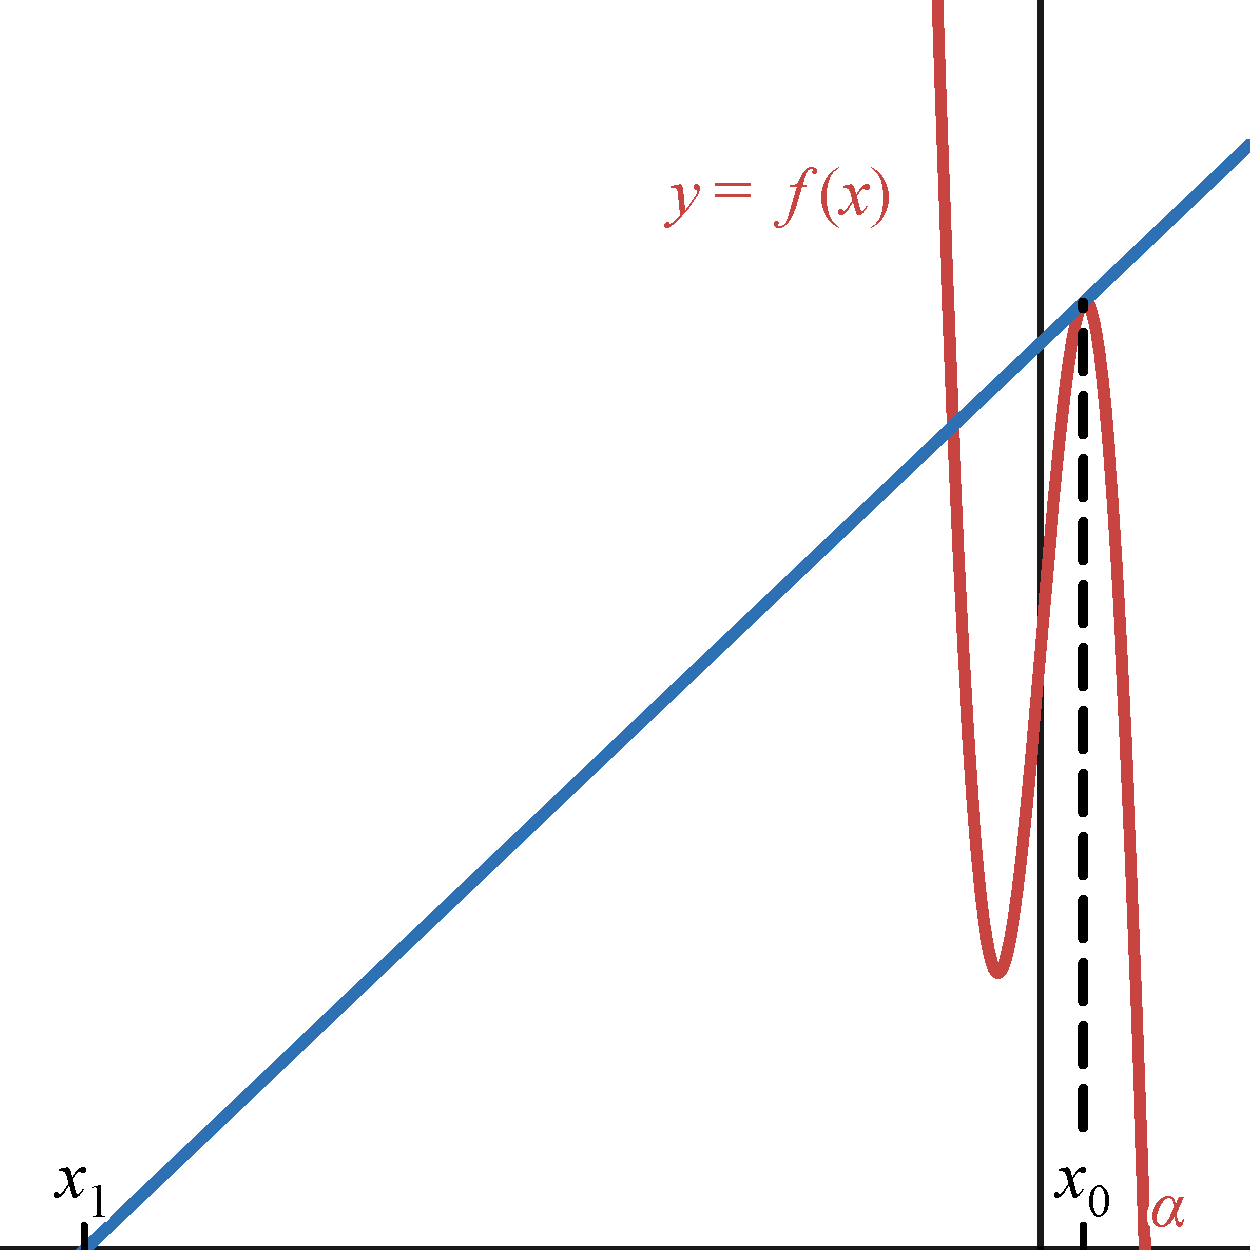
\includegraphics[width=0.5\textwidth]{../Diagrams/newton's-method-prelim.pdf}
        \caption{\ref{Me} \href{https://www.desmos.com/calculator/mq2elll5k3}{(Desmos)}}
        \label{fig:newton's-method-prelims}
    \end{figure}
    \begin{enumerate}
        \item Since \(x_0=\rule{0.5cm}{0.05mm}\) is very close to the stationary point, the tangent to the curve \(y=f(x)\) has a very gentle gradient. Thus, it cuts the \(x\)-axis far away from the initial approximation. 
        \item Furthermore, as \(x_0=\rule{0.5cm}{0.05mm}\) is to the left/right of the minimum/maximum point \(x=\rule{0.5cm}{0.05mm}\), the values of the gradient \(f'(x_n)\) will be negative/positive for all \(n\geq 0\). Hence, \(x_n\) converges to the root \(\beta\) instead \(\alpha\). 
    \end{enumerate}
    (The second point may be omitted if it is irrelevant.)
\end{note}
\begin{note}
    Suppose a question asks for the approximation of a root to \(k\) significant figures/\(k\) decimal places. Then: 
    \begin{enumerate}
        \item We leave our iterative approximations \(x_n\) to at least \(k+2\) significant figures/\(k+2\) decimal places.
        \item We continue the iterative process till two consecutive ones agree up to \(k\) significant figures/\(k\) decimal places.
    \end{enumerate}
\end{note}
\begin{note}
    Perform \rule{1.5cm}{0.01mm} (e.g. linear interpolation) to obtain an approximation for \(\alpha\), correct to two decimal places. Justify whether this approximation is sufficiently accurate.

    \rule{20cm-137.0549pt}{0.05mm}
    
    \vspace{0.5\baselineskip} Suppose our approximation is some \(a=1.00\), then we note the sign of \(f\) at \(a\pm 0.\highlight[yellow]{00}5\). (For an arbitrary number of s.f. or d.p., simply adjust the value \(0.\highlight[yellow]{00}5\) accordingly. E.g. for 3 d.p. we instead use \(0.\highlight[yellow]{000}5\)). Our working should look similar to the following:
    \begin{center}
        \parbox{0.9\textwidth}{
            Since \(f(0.995)=\rule{0.5cm}{0.01mm}<0\) and \(f(1.005)=\rule{0.5cm}{0.01mm}>0\), we conclude that \(1.00\) is a sufficiently accurate approximation, at 2 d.p..
        }
    \end{center}
\end{note}
\begin{note}
    The \emph{error obtained} when using an approximation should be the \emph{absolute} difference of the true value and the approximation. 
\end{note}
\begin{note}
    Use the results of part (i) and the differential equation \(dy/dx=\sin(xy)\) to estimate the \(x\)-coordinate \(x_P\) of \(P\). 

    \rule{20cm-137.0549pt}{0.05mm}

    \vspace{0.5\baselineskip} The maximum point occurs when \(dy/dx=\sin(xy)=0\), i.e. \(xy=k\pi\) where \(k\in \mathbb{Z}\). From (i), \(\frac{dy}{dx}\big|_{x=5/3}\approx 0.643>0\) so \(y_P>y(5/3)\approx 2.0468\). Hence, \(x_P\approx \pi/2.04679402=1.53\) (3.s.f).
\end{note}
\begin{GCSkills}{}
    Linear interpolation: finding an approximation to a root in \([a,b]\) up to \(n\) decimal places.
    \begin{enumerate}
        \item \(Y_1=f(x)\),
        \item \(a \to A\) and \(b \to B\),
        \item \(\dfrac{B \lvert Y_1(A) \rvert+A \lvert Y_1(B) \rvert}{\lvert Y_1(A) \rvert+\lvert Y_1(B) \rvert}\),
        \item \(\text{Ans}\to A \text{ or } B\) (choose the one that has the opposite sign to Ans),
        \item Repeat steps 4 to 5,
        \item Terminate this process when the approximations are consistent up to \(n\) decimal places.
    \end{enumerate}
    \end{GCSkills}
    You can freely enter any function and shift the initial values in the Desmos graphs below!
    \newpage
    \begin{figure}[H]
        \centering
        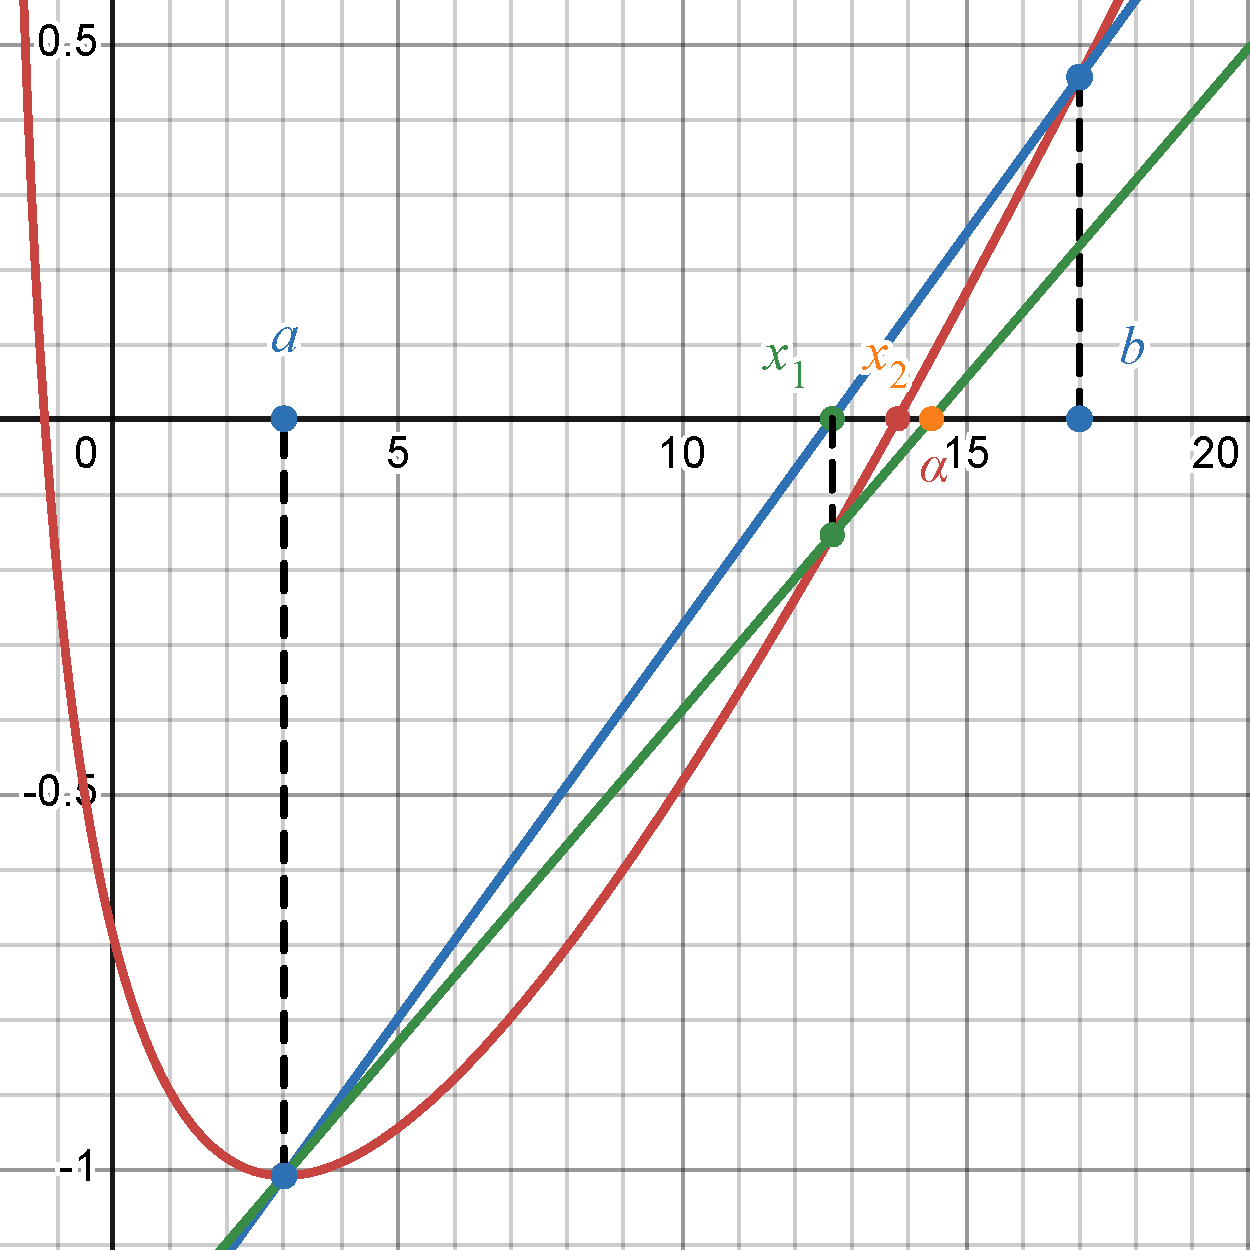
\includegraphics[width=0.69\textwidth]{../Diagrams/linear-interpolation.pdf}
        \caption{\ref{Me} An illustration of linear interpolation \href{https://www.desmos.com/calculator/yz71wfvkrl}{(Desmos)}.}
        \label{fig:linear-interpolation}
        % The second and third lines are wrong! 
    \end{figure}
    \begin{figure}[H]
        \centering
        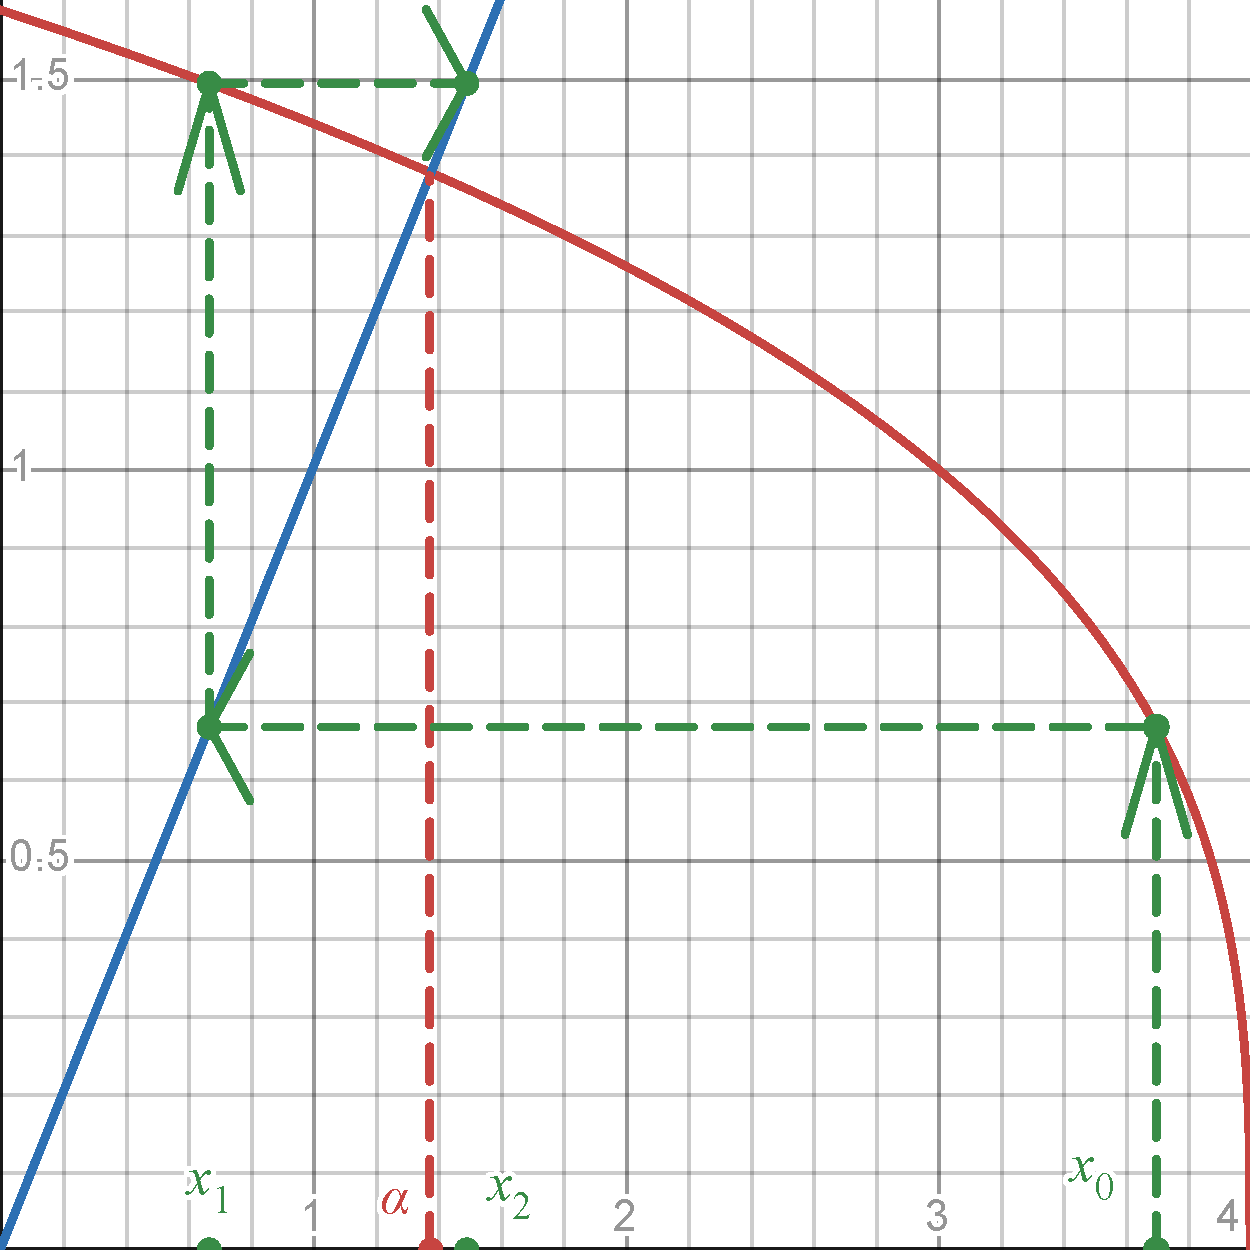
\includegraphics[width=0.69\textwidth]{../Diagrams/fixed-point-iteration/fixed-point-iteration-desmos.pdf}
        \caption{\ref{Me} An illustration of fixed-point iteration \href{https://www.desmos.com/calculator/t9mnqtmhxw}{(Desmos)}.}
        \label{fig:fixed-point-iteration}
    \end{figure}
    % \begin{figure}[H]
    %     \centering
    %     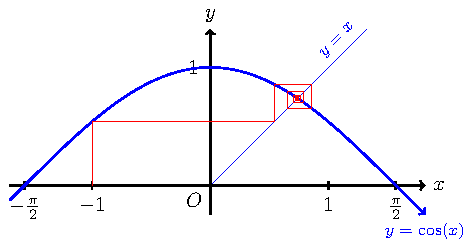
\includegraphics[width=\textwidth]{../Diagrams/fixed-point-iteration/fixed-point-iteration.pdf}
    %     \caption{An illustration of fixed-point iteration.}
    %     \label{fig:fixed-point-iteration}
    % \end{figure}
    \begin{figure}[H]
        \centering
        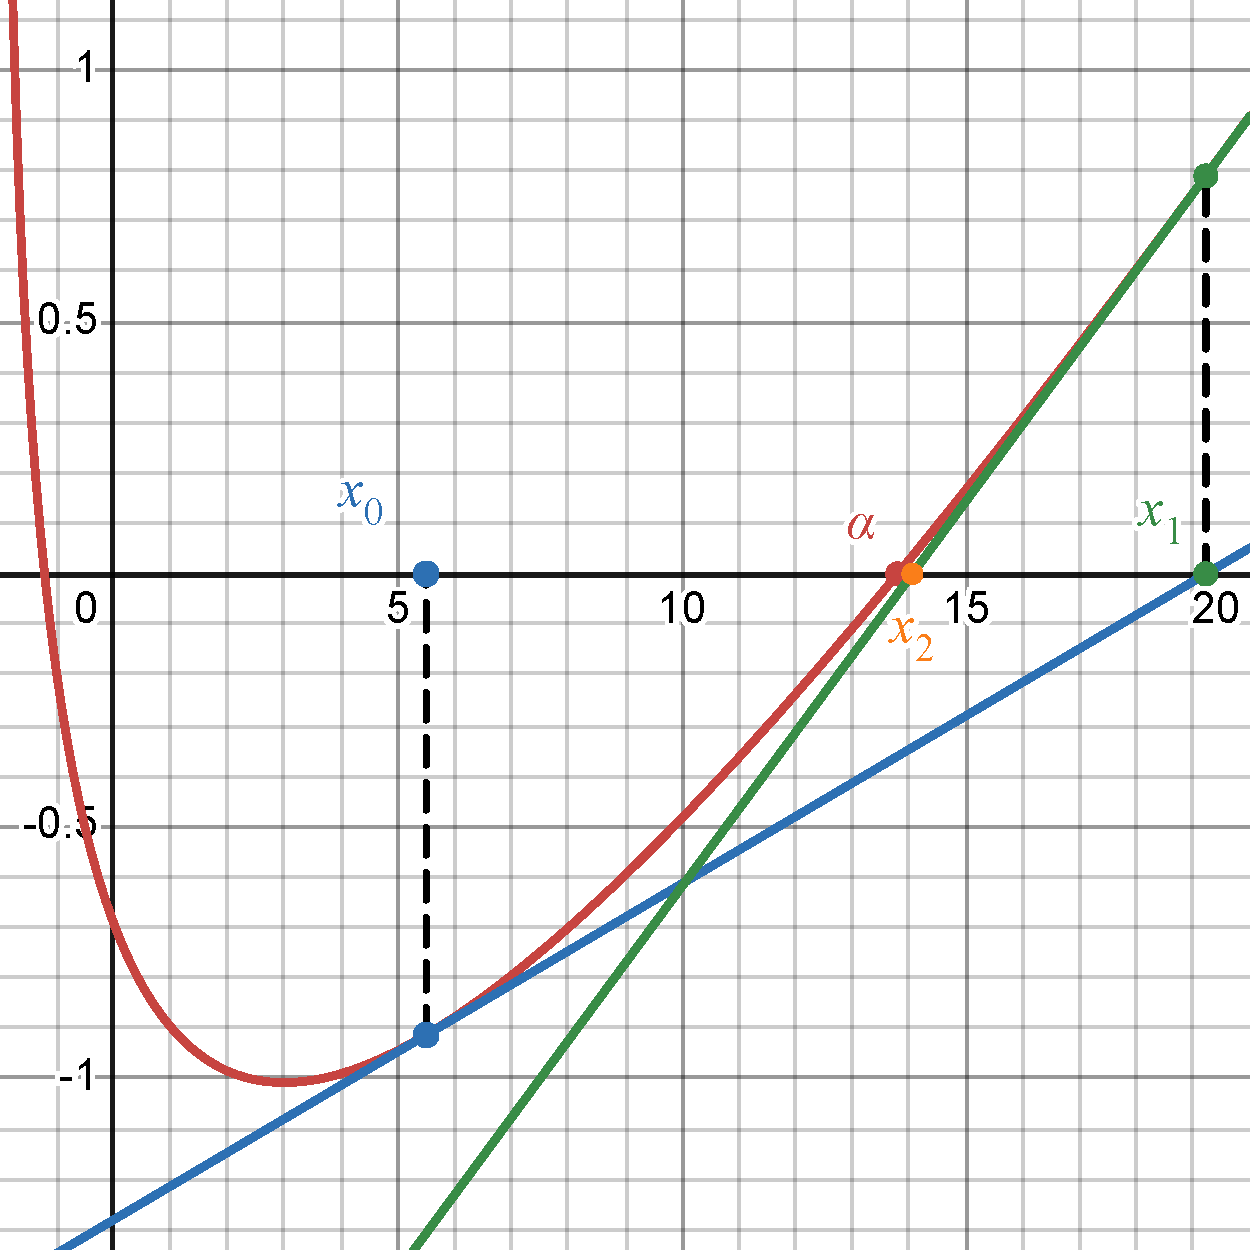
\includegraphics[width=0.69\textwidth]{../Diagrams/newton's-method.pdf}
        \caption{\ref{Me} An illustration of Newton's Method \href{https://www.desmos.com/calculator/izkg4ynlfp}{(Desmos)}.}
        \label{fig:newton's-method}
    \end{figure}